\part{Ziel der Dokumentation}
\label{Ziel der Dokumentation}
\section{Bedeutung von Remote Logging}
Durch den hohen Zeitdruck, stetig wachsender Aufgabenkomplexität und täglich steigender Serverkapazität ist es den System-Administration meist nicht mehr möglich alle Server im Überblick zu behalten. Hierzu kommt das Problem dass man sich auf jeden Server verbinden muss, um Log-Datein einsehen zu können. Somit bietet für System Administratoren das Protokollieren aller Servernachrichten an einer Zentralen stelle viele Vorteile.

\section{Aufbau diese Dokumentation}
Diese Dokumentation beschreibt unter anderem die Verwendung von \textit{rsyslog} in Zusammenarbeit mit \textit{tenshi} und \textit{phpLogCon}. Hierzu wird von folgendem Aufbau ausgegangen.

\begin{figure}[h]
\begin{center}
 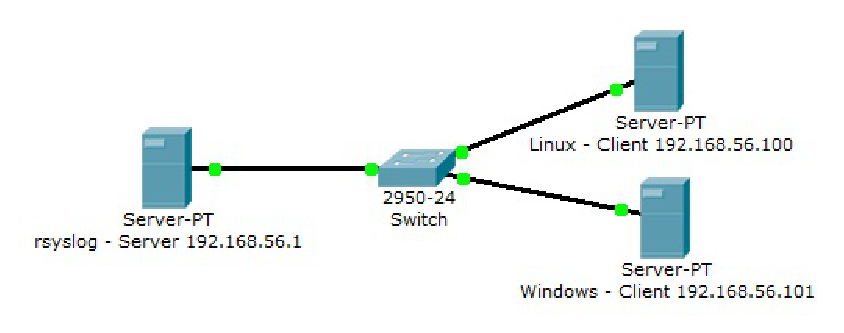
\includegraphics[width=\textwidth]{content/images/Server-Aufbau.eps}
  \caption{Konfiguration, Aufbau}
\end{center}
\end{figure}

In dieser Dokumentation wird von einem Grundverständnis für das syslog-Protokoll ausgegangen.

In Teil II werden die Basisdienste, ihre Vorteile und Alternativen vorgestellt. Für erfahrene System-Administratoren bietet Teil III eine genaue Erklärung der Konfiguration.

\section{Informationen zur Konfiguration}
% TODO: Dokumentation und Konfiguration hochladen (Projekt anlegen)
Die komplette Dokumentation inklusive aller Konfigurationsdateien befindet sich auf \url{https://github.com/drscream/rsyslog-workshop}. Als Linux Distribution wird Ubuntu Server 10.04 LTS eingesetzt, die Konfiguration kann daher zu anderen Linux Derivaten abweichen.
